% Template for Cogsci submission with R Markdown

% Stuff changed from original Markdown PLOS Template
\documentclass[10pt, letterpaper]{article}

\usepackage{cogsci}
\usepackage{pslatex}
\usepackage{float}

% amsmath package, useful for mathematical formulas
\usepackage{amsmath}

% amssymb package, useful for mathematical symbols
\usepackage{amssymb}

% hyperref package, useful for hyperlinks
\usepackage{hyperref}

% graphicx package, useful for including eps and pdf graphics
% include graphics with the command \includegraphics
\usepackage{graphicx}

% Sweave(-like)
\usepackage{fancyvrb}
\DefineVerbatimEnvironment{Sinput}{Verbatim}{fontshape=sl}
\DefineVerbatimEnvironment{Soutput}{Verbatim}{}
\DefineVerbatimEnvironment{Scode}{Verbatim}{fontshape=sl}
\newenvironment{Schunk}{}{}
\DefineVerbatimEnvironment{Code}{Verbatim}{}
\DefineVerbatimEnvironment{CodeInput}{Verbatim}{fontshape=sl}
\DefineVerbatimEnvironment{CodeOutput}{Verbatim}{}
\newenvironment{CodeChunk}{}{}

% cite package, to clean up citations in the main text. Do not remove.
\usepackage{cite}

\usepackage{color}

% Use doublespacing - comment out for single spacing
%\usepackage{setspace}
%\doublespacing


% % Text layout
% \topmargin 0.0cm
% \oddsidemargin 0.5cm
% \evensidemargin 0.5cm
% \textwidth 16cm
% \textheight 21cm

\title{Understanding when active learning is most effectivne}


\author{{\large \bf Kyle MacDonald} \\ \texttt{kyle.macdonald@university.edu} \\ Department of Psychology \\ Stanford University \And {\large \bf Michael C. Frank} \\ \texttt{mcfrank@university.edu} \\ Department of Psychology \\ Stanford University}

\begin{document}

\maketitle

\begin{abstract}
Active learning contexts can speed knowledge acquisition by allowing
people to select highly informative examples based on their prior
experience. But real-world learning often involves both active and
passive training, an interaction that we know little about. Moreover,
work in machine learning shows that active learning systems can perform
worse than random sampling when starting with the wrong initial
hypothesis. In two large-scale experiments with adults, we test the
effect of order of active/passive training (Experiment 1) and the
quality of the learner's initial hypothesis (Experiment 2) on the
effectiveness of active learning in a category learning task. Across all
experiments, active training resulted in better category learning
compared to passive learning. Classification accuracy was better when
people received passive training before active training. Finally,
learning was hindered when there was mismatch between the learner's
prior hypotheses and the target category structure. The overall pattern
of results did not change when learning a more or less complex category
structure. Our data provide additional support that active learning
provides an advantage over passive learning. But our results extend
these findings to show that active learning is more effective when the
learner already has some experience with the task and when they were
considering the correct initial hypothesis.

\textbf{Keywords:}
active learning, hypothesis testing, cognitive development, replication
\end{abstract}

\section{Introduction}\label{introduction}

*What is active learning?

*Why is active learning helpful?

\emph{Brief literature review } Human active * Machine active learning *
When is active learning most effective

*Current work

Questions for Mike: \emph{Do we present the replication as a separate
study? Do we emphasize the replication? }Framing --\textgreater{}
interaction between active/passive learning? when is active learning
effective?

\section{Experiment 1}\label{experiment-1}

\subsection{Methods}\label{methods}

\subsubsection{Participants}\label{participants}

We posted a set of Human Intelligence Tasks (HITs) to Amazon Mechanical
Turk. Only participants with US IP addresses and a task approval rate
above 85\% were allowed to participate, and each HIT paid one dollar.
TODO HITs were posted for each of the TODO between-subjects conditions.
Data were excluded if participants completed the task more than once or
if they reported that they did not understand the task at the end of the
experiment (TODO HITs). The final sample consisted of TODO participants.

\subsubsection{Stimuli}\label{stimuli}

\begin{CodeChunk}
\begin{figure}[tb]

{\centering 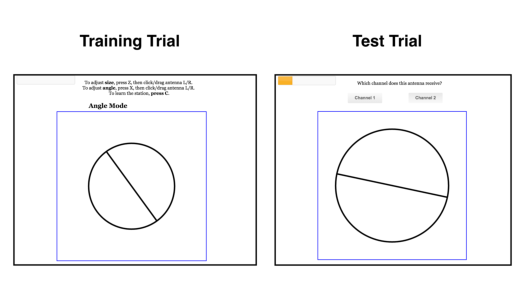
\includegraphics{figs/stimuli-1} 

}

\caption[Screenshots of training and test trials used in all Experiments]{Screenshots of training and test trials used in all Experiments. In the Active training condition, participants could interact with the antenna by adjusting it's size and/or angle. In the Passive training condition, participants saw an antenna and were told which channel it received. Test trials were identical across all conditions.}\label{fig:stimuli}
\end{figure}
\end{CodeChunk}

\subsubsection{Design and procedure}\label{design-and-procedure}

\subsection{Results and Discussion}\label{results-and-discussion}

\section{Experiment 2}\label{experiment-2}

\subsection{Methods}\label{methods-1}

\subsubsection{Participants}\label{participants-1}

Participant recruitment and inclusionary/exclusionary criteria were
identical to those of Experiment 1 (excluded TODO HITs). TODO HITs were
posted for each condition (TODO) for total of TODO paid HITs.

\subsubsection{Design and procedure}\label{design-and-procedure-1}

\subsection{Results and Discussion}\label{results-and-discussion-1}

\section{Experiment 3}\label{experiment-3}

\subsection{Methods}\label{methods-2}

\subsubsection{Participants}\label{participants-2}

\subsubsection{Design and procedure}\label{design-and-procedure-2}

\subsection{Results and Discussion}\label{results-and-discussion-2}

\section{General Discussion}\label{general-discussion}

\begin{CodeChunk}
\begin{figure}[H]
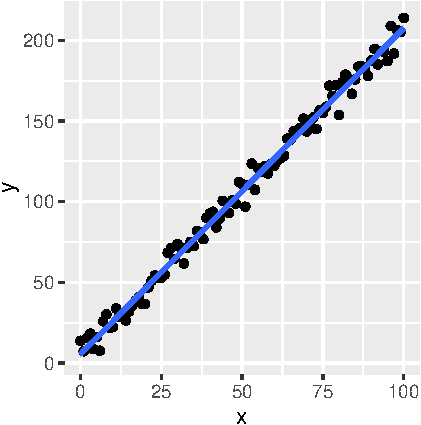
\includegraphics{figs/plot-1} \caption[R plot]{R plot}\label{fig:plot}
\end{figure}
\end{CodeChunk}

\begin{table}[H]
\centering
\begin{tabular}{rrrrr}
  \hline
 & Estimate & Std. Error & t value & Pr($>$$|$t$|$) \\ 
  \hline
(Intercept) & -0.05 & 0.11 & -0.5 & 0.61 \\ 
  x & 2.02 & 0.11 & 18.7 & 0.00 \\ 
   \hline
\end{tabular}
\end{table}

\section{Acknowledgements}\label{acknowledgements}

We are grateful to Doug Markant and Todd Gureckis for sharing their data
and the details of the original experiment. We thank the members of the
Language and Cognition Lab for their helpful feedback on this project.
This work was supported by a National Science Foundation Graduate
Research Fellowship to KM.

\section{References}\label{references}

\setlength{\parindent}{-0.1in} \setlength{\leftskip}{0.125in} \noindent

\end{document}
